\section{Background}
\label{sec:background}

The training of LLMs, characterized by their vast model architectures and
massive datasets, is computationally intensive. Parallelism strategies
distribute the training process across multiple devices.

\begin{figure}
    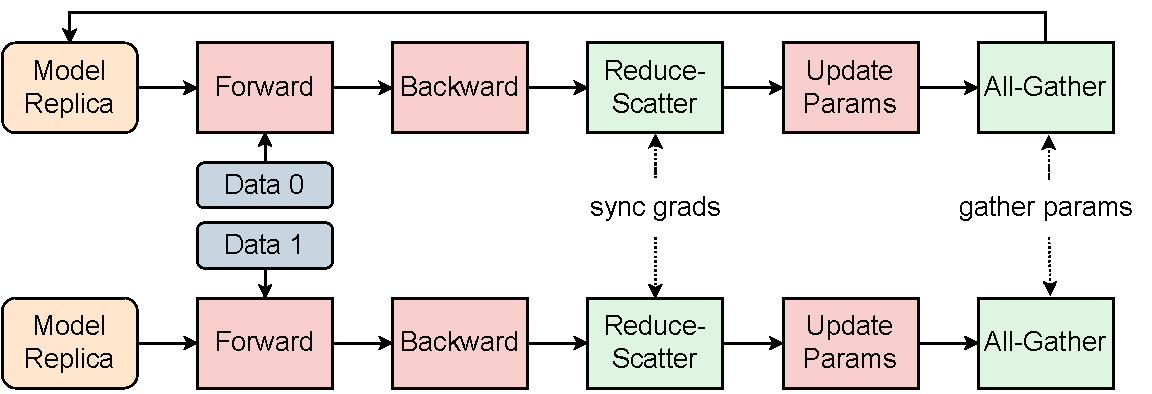
\includegraphics[width=0.49\textwidth]{figures/background/dp-zero.pdf}
    \caption{Data parallel training with ZeRO2.}
    \label{fig:dp-zero}
\end{figure}

\parabf{Data parallelism.} It replicates the model and optimizer states across
multiple devices and the data is evenly divided among all devices. Each model
replica executes the forward and backward propagation computation in parallel.
Upon completion of each iteration, all model replicas synchronize to update the
model. Instead of duplicating model states (like the optimizer states,
gradients, and parameters), Zero Redundancy Optimizer (ZeRO) \cite{zero} shards these states
across every data-parallel process. As a result, the traditional all-reduce
operations that aggregate gradients are decomposed into separate reduce-scatter
and all-gather operations. This is because every data-parallel process retains
only a fraction of the total state. ZeRO is structured into three incremental
stages of optimizations. Notably, the second stage is commonly adopted to shard
both the optimizer states and gradients, while ensuring no additional
communication overhead is introduced (Figure~\ref{fig:dp-zero}).

\parabf{Pipeline parallelism.} It distributes model layers among multiple
devices and each  device owns a portion of the model. Meanwhile, each training
batch is subdivided into a number of micro-batches for pipelined execution. To
reduce pipeline bubbles, various pipeline scheduling strategies are proposed,
e.g., GPipe~\cite{huang2019gpipe}, PipeDream 1F1B~\cite{pipedream}, etc. Megatron-LM~\cite{narayanan2021efficient} employs
the interleaved 1F1B scheduling. Each pipeline stage on every worker is
subdivided into multiple virtual stages, which represents a subset of layers,
referred to as a model chunk. Initially, workers enter a \textit{warm-up} phase,
executing the forward pass for a limited number of in-flight micro-batches.
Following the warm-up, each worker progresses to the \textit{steady} phase where
workers perform one forward pass followed by one backward pass, often
abbreviated as 1F1B. Upon concluding a batch, workers finalize the backward
passes for any remaining in-flight micro-batches during this \textit{cool-down}
phase. Figure~\ref{fig:pipeline} shows an three-stage pipeline where each stage is
further divided into two virtual stages.

\begin{figure}
    
\includegraphics[width=0.46\textwidth]{figures/background/pipeline.pdf}
    \caption{Interleaved 1F1B pipeline.}
    \label{fig:pipeline}
\end{figure}

\parabf{Tensor parallelism.} It distributes individual operators over multiple
devices, with each device executing a portion of the computation in parallel.
Depending on the specific partitioning strategy and its relationship to prior
and subsequent operators in the model, partitioning can require communication
among participating GPUs to split the input and then merge the output. For example, we
can split GEMMs in the MLP and self-attention blocks among multiple GPUs to
utilize more computational units. Some other operations like LayerNorm and
Dropout are less computationally intensive but demand a considerable amount of
activation memory. Another form of tensor parallelism called sequence parallelism is
proposed to distribute these operators along the sequence dimension to
effectively reduce the activation memory footprint.

\parabf{Combination of parallelism strategies.}
These parallelism strategies can be combined into 3D parallelism to scale the
training of LLMs across many GPUs~\cite{shoeybi2020megatronlm}. Given the high
communication overhead associated with tensor parallelism, it is preferable to
confine such communication within a single cluster node. Conversely, data
parallelism and pipeline parallelism are more amenable to inter-node
communication. In this case, we choose to prioritize building the data
parallelism groups over pipeline parallelism, which can mitigate cross-minipod
communication for data parallelism. 